% !TEX TS-program = xelatex
%
\documentclass[a4paper]{scrartcl}

\usepackage{lmodern}

\usepackage[english]{babel}

\usepackage{xcolor}
\usepackage{listings}

\lstset{basicstyle=\ttfamily,
  breaklines = true,
  showstringspaces = false,
  commentstyle=\color{red},
  keywordstyle=\color{blue}
}

\usepackage[
% style   = numeric,
  style   = alphabetic,
% style   = authortitle,
% style   = verbose,
% style   = reading,
% style   = draft,
  sorting = none,
]{biblatex}
\bibliography{thesis}

\usepackage{bookmark}
\usepackage{hyperref}

\usepackage{graphicx}
\usepackage{graphbox}
\graphicspath{ {../assets/} }

\title{IoT Data Analytics using Serverless Computing - Raspberry Pi}

\author{Markus Reiter, Michael Kaltschmid}
\date{}

\begin{document}
  \maketitle

  \section*{Abstract}

Cloud computing in the grand scheme of things is still a relative new development, which has seen
rapid growth in recent years and with that has seen a lot of technologies around it. One of those is
the concept of \textit{Serverless Computing} or \textit{Function as a Service (FaaS)}. Due to its
versatile nature, a lot of big players in the cloud computing field jumped on it and have their own
implementation in their portfolio.

Same as with the \textit{cloud}, the \textit{Internet of Things (IoT)} has also seen large adoption
in many aspects of life and are an integral part of it. May it be for household appliances or in the
industry. \textit{IoT} devices can be found everywhere.

This bachelor tries to show the usefulness of \textit{Serverless Computing} in conjunction with
\textit{IoT} devices by building a infrastructure to host these \textit{serverless functions}, where
then all \textit{IoT} devices can send their data to. While not a classic \textit{IoT} device there
is also support for phones on both \textit{Android} and \textit{iOS} to transmit data. This data is
then further used for analytics and visualised with graphs in a \textit{Web UI}. In order to achieve
this we decided to use the framework \textit{OpenFaaS} to realise the hosting function platform.
Furthermore \textit{Kafka} is used to manage all incoming requests from devices. \textit{Kafka} also
handles the forwarding of requests to functions. For persistence of sensor data we have the
\textit{NoSQL} database \textit{MongoDB}. The database is of great health when confronted with data
of \textit{IoT} devices. Having a stack like this also means to deal with a lot of configuration. To
aid the process of deployment with a \textit{Rake} script which makes everything runnable with only
one command and finally \textit{Azure Pipelines} as our verification tool. With it we can test all
parts of our stack and even push the images of functions to a online registry, which makes
deployment even faster.

In the final chapter of the thesis we also have results regarding function by measuring the latency
of requests. In addition to that we also provide benchmarks for the startup time of our whole stack,
where we compare the time to be up and running by building all function on the target machine first,
with the optimised way of fetching all function images from the registry.


  \newpage
  \tableofcontents

  \newpage
  \chapter*{Preface}

This thesis was conducted by two students. The tasks of the implementation as well as those of
writing the thesis were distributed evenly between both members of the team.

The following shows the contributions of each member regarding the implementation in more detail:

\begin{itemize}
  \setlength\itemsep{-1em}
  \item \textit{Rasperry Pi} application and wiring: \textbf{mostly Markus}
  \item \textit{Serverless Functions}: \textbf{mostly Markus}
  \item Developing the \textit{OpenFaaS} stack and its core components: \textbf{Markus and Michael}
  \item Mobile application: \textbf{mostly Michael}
  \item \textit{Serverless UI}: \textbf{mostly Michael}
\end{itemize}

The following shows the contributions of each member regarding the written part in more detail:

\begin{itemize}
  \setlength\itemsep{-1em}
  \item \Cref{sec:introduction} \nameref{sec:introduction}: \textbf{Markus and Michael}
  \item \Cref{sec:background} \nameref{sec:background}: \textbf{Markus and Michael}
  \item \Cref{sec:motivation} \nameref{sec:motivation} \textit{Motivation}: \textbf{Markus and Michael}
  \item \Cref{sec:implementation} \nameref{sec:implementation}: \textbf{Markus and Michael}
  \item \Cref{sec:results} \nameref{sec:results}: \textbf{Markus and Michael}
  \item \Cref{sec:conclusion} \nameref{sec:conclusion}: \textbf{Markus and Michael}
\end{itemize}

In all the parts where one member has done most of the work, the other member of the team has
thoroughly verified the work and agreed on the implementation or writing details.


  \newpage
  \chapter{Introduction}
\label{sec:introduction}

In recent years, the number of IoT (Internet of Things) devices has been growing continuously.
Naturally, all of these devices generate a lot of data. This usually happens asynchronously, which
means that a normal server processing this data would either be under or overutilised. A well known
method to deal with this kind of problem is to use the \textit{edge-fog-cloud} approach to process
data earlier, either on an edge device itself or on a fog device instead of doing all processing in
the cloud, which can have noticeable performance benefits. This is where \textit{serverless
computing} comes into play. In contrast to traditional software development where the software is
centred around a single server delivering all of the functionality. \textit{Serverless computing} is
based around the idea of splitting this functionality into separate functions, which is especially
beneficial when dealing with many IoT devices, since functions can be scaled individually according
to the current utilisation and can be started on demand. This results in more efficient usage of
resources and improved modularity.

Today IoT devices can be found in household appliances like washing machines, fridges, televisions,
garage doors and many more. For this thesis, their application for the purpose of data collection
was our primary focus. A big advantage to using IoT devices is the low cost of some of the
do-it-yourself and \textit{open source} solutions, which can be achieved with a
\textit{micro-controller} such as the \textit{Raspberry Pi} and readily available
\whitelist{off-the-shelf} sensors.

In this thesis, we explore the possibility of combining both \textit{serverless computing} and IoT
for the purpose of analysing sensor data. More specifically, we want to test the limits of cheap IoT
hardware in a \textit{serverless} context. Furthermore, we want to subsequently visualise the
collected data in an intuitive user interface that can be displayed on any device.

The end result of this thesis is a system which can be used to collect sensor data from IoT devices
using a \textit{serverless} architecture and an accompanying web interface to visualise the
collected data. In the following sections we explain the technologies used, a more detailed
explanation about the motivation for using \textit{serverless computing} as well as how the
different parts of our project were implemented. Finally, we provide some results on how our system
performs when running on affordable hardware.

  \section{Motivation}
\label{sec:motivation}

In this section, we describe our motivation for exploring IoT data analysis using serverless
computing.

\subsection{Flexibility}

Using a serverless approach for building software inherently provides more flexibility than the
traditional approach of using a monolithic architecture. This applies to both the development
process itself as well as the much more diverse deployment options presented by serverless
computing. Traditionally, you would have to choose a single programming language for a project since
using multiple would increase complexity of both the development phase as well as the deployment
strategy. Also, the initial setup of a single server and its ongoing maintenance for use with only a
single language is much easier than having to maintain a server running multiple different
languages. In this regard, serverless computing provides much greater flexibility.

A serverless program is built from separate functions interacting with one another. These functions
usually communicate via a JSON API. Functions are programming language agnostic, so as long as the
language you are using can invoke or receive web requests, you can use it to develop a function.
This gives the developer the freedom to choose the best language for a given task, rather than
sticking to a single language which might not be ideal for some specific tasks. Additionally,
deployment of functions is managed by the serverless stack, so once the serverless stack is
deployed, there is no more maintenance overhead.

Every function is a self-contained unit of execution, usually in the form of a container which can
be deployed on the serverless stack. This means that the programming language runtime environment
and all dependencies are contained in a single container. This allows the developer to not only use
different programming languages but also different versions of the same language without any
maintenance difficulties or conflicts compared to doing the same on a single server.

\subsection{Modularity}

The traditional approach of a monolithic architecture is by nature error prone and not failure
tolerant. If one component crashes, all other components on that server might go down as well. With
serverless functions, this problem can be avoided as every function is an individual item and
therefore isolated from other functions. This fact makes maintaining systems much easier as problems
are faster and more efficient to identify. Testing is also simpler as tests can be written for
individual functions instead of for chunks in a larger code base.

\subsection{Efficiency}

Traditional software stacks often require considerable hardware in order to run software
efficiently. In our thesis we try to show that rich functionality on the server side can also be
achieved without expensive hardware with the power of serverless computing. Since the heavy lifting
is done by the serverless stack and the clients in our case only have to read sensor data and invoke
web requests, almost any cheap micro-controller is sufficient for processing.

\subsection{Portability}

Another one of the advantages of serverless computing is portability as one can easily transfer all
functions from one provider to another. In our case however, we try to take things further as not
only the functions are portable, the whole stack in a sense is portable. Every major component of
the stack is composed of containers, which means as long as \textit{Docker} is installed on the host
machine, the stack should be able to run on it.

  \chapter{Background}
\label{sec:background}

Since we use many different technologies, we briefly present each of them in this section in order
to make the reader more familiar with the individual technologies and their respective terms that
will be used throughout the thesis. Firstly we start by discussing the main topic,
Serverless Computing. We will then go on in more detail about \textit{Docker} and our
specific use case.

\section{Serverless Computing}

Serverless computing is a new emerging paradigm for deploying applications into the cloud. It gained
in popularity in recent years largely due to shift of enterprise application deployment in
containers and microservices. Serverless Computing offers developers a simplified
programming model for creating cloud applications while minimising operational concerns.
\cite{servprog}

The name “serverless computing” is not quite fitting, since physical server hardware is of course
still needed in order to run applications. The main point is that the application user or developer
does not need to manage scaling, plan for variable capacity or maintain any other aspect of the
servers. The management of all of these things is provided as a service from the cloud provider.
\cite{wikiservcomp}

\subsection{Layers of Cloud Computing}

\begin{figure}[H]
  \centering
  \adjincludegraphics[max width=\textwidth]{cloud-history}
  \caption{History of cloud computing: going from Data Centre to IaaS, to PaaS, to finally
  Serverless (FaaS) \cite{layercloudcomp}}
\end{figure}

Historically, each new paradigm in the space of cloud computing has brought with it a new layer of
abstraction. First, there was the move from managing physical hardware in a data centre to being
able to rent infrastructure from a cloud provider. This layer, called IaaS (Infrastructure as a
Service), shifted the need for the customer to manage hardware infrastructure onto the cloud
provider. This change also improved scalability as customers could now rent infrastructure based on
the pay-as-you-go principle instead of paying for large servers which would be idle most of the
time.

With IaaS, the customer is still responsible for managing the setup of the rented infrastructure,
i.e. installing the necessary dependencies needed to run a given application. Naturally, the next
layer of abstraction is to provide the customer with an environment suited to run an application
without the need to manually install a programming language or any dependencies. This layer is
called PaaS (Platform as a Service). Using this layer of abstraction, the user does have to worry
neither about managing the underlying hardware nor about managing the operating system the
application is running on.

Now, in the era of serverless computing, there is yet again a new layer of abstraction. Called FaaS
(Function as a Service), this layer provides a runtime environment for a given language in which to
run individual functions in. An application deployed in a FaaS environment consists of multiple
functions interacting with one another whereas in a PaaS environment, an application is deployed as
a single unit.

\subsection{Functions}

A serverless program is built from separate functions interacting with one another. These functions
usually communicate via a JSON API. Functions are programming language agnostic, so as long as the
language you are using can invoke or receive web requests, you can use it to develop a function.
This gives the developer the freedom to choose the best language for a given task, rather than
sticking to a single language which might not be ideal for some specific tasks. Additionally,
deployment of functions is managed by the serverless stack, so once the serverless stack is
deployed, there is no more maintenance overhead.

Every function is a self-contained unit of execution, usually in the form of a container which can
be deployed on the serverless stack. This means that the programming language runtime environment
and all dependencies are contained in a single container. The developer then has the ability to not
only use different programming languages but also different versions of the same language without
any maintenance difficulties or conflicts compared to doing the same on a single server.

\section{Docker}

Docker is a technology which is used to run software packaged into containers. Containers are
self-contained and provide an isolated environment for software to run in. A container includes all
configuration files and dependencies as well as the software itself, which makes it highly portable.
In the case of \textit{Docker}, these stand-alone container images can then be executed by the
\textit{Docker Engine}, which turns the stored images into running containers. For this reason,
every container image contains a customisable \textit{entry point} command which is executed when
the container is started.

\begin{figure}[H]
  \centering
  \adjincludegraphics[max width=\textwidth]{docker-containerized-and-vm}
  \caption{Comparison of Containerised Applications and Virtual Machines \cite{docker-container}}
\end{figure}

\textit{Docker} containers are standardised, which means they can run virtually anywhere the
\textit{Docker Engine} is supported, be it on Linux, Windows, in data centres or in the cloud.
Compared to virtual machines, containers are very lightweight since they share the host machine's
system kernel and thus don't require a separate operating system for each application. Despite not
using a separate operating system, containers are completely isolated from the host system as well
as other containers by default.

Furthermore, since containers usually don't contain a full operating system, startup times are also
much faster compared to virtual machines, which have to completely boot the entire operating system
from scratch in addition to starting the application. \cite{docker-container}

\section{OpenFaaS}

“OpenFaaS – Serverless Functions Made Simple”. As the slogan already entails, \textit{OpenFaaS} is a
framework for the deployment of serverless functions. In contrast to competing hosted products like
\textit{AWS Lambda} or \textit{Azure Cloud Functions}, it offers a lot more flexibility regarding
the way functions are written and hardware resources are managed. In fact, any programming language
imaginable can be used to write functions for \textit{OpenFaaS}, as long as that language can run or
be compiled in a \textit{Docker} container. Deploying an \textit{OpenFaaS} stack in a cluster is
easy as well, as the framework poses itself for having first class support for \textit{Docker Swarm}
and being \textit{Kubernetes} native. \cite{openfaas-docs}

\begin{figure}[H]
  \centering
  \adjincludegraphics[max width=\textwidth]{of-workflow}
  \caption{\textit{OpenFaaS} workflow \cite{openfaas-docs}}
\end{figure}

\section{MongoDB}

\textit{MongoDB} is a document database that is scalable and flexible. The data in a
\textit{MongoDB} database is stored in flexible, \textit{JSON}-like documents, making it easy to
work with. The document database offers powerful ways to access and analyse data with features like
ad hoc querying and real time aggregation. Since \textit{MongoDB} is a distributed database at its
core, high availability and horizontal scaling are already built in. Furthermore, due to its
“real-time” nature, \textit{MongoDB} lends itself very well for \textit{IoT} applications.
\cite{mongodb-description}

\begin{code}[H]
  \centering
  \begin{lstlisting}[language=mongo]
{
  _id: '5cf0029caff5056591b0ce7d',
  name: 'Jane Wu',
  address: {
    street: '1 Circle Rd',
    city: 'Los Angeles',
  }
}
  \end{lstlisting}
  \caption{A \textit{MongoDB} document (adapted from \cite{mongodb-description}).}
\end{code}

\section{Apache \whitelist{ZooKeeper}}
\label{sec:background-zookeeper}

\textit{ZooKeeper} is a service for centrally managing configuration, naming, handling distributed
synchronisation and providing group services. Many distributed applications need access to some or
all of these kinds of services, so \textit{ZooKeeper} is a great way to avoid reinventing the wheel
in that respect. This is especially true given the fact that these highly distributed scenarios
bring with them a vast amount of potential bugs and race conditions every time these services would
have to be implemented from scratch. It is incredibly hard to get these things completely right the
first time and by using \textit{ZooKeeper}, all of these potential problems are nullified and a lot
of time can be saved which can consequently be spent developing the actual application logic rather
than spending it on debugging synchronisation problems or managing configuration across a
distributed network. Particularly in the long run, using \textit{ZooKeeper} helps reduce unforeseen
complexity for applications continuously increasing in size.
\cite{zookeeper-homepage}

\section{Apache Kafka}
\label{sec:background-kafka}

\textit{Apache Kafka} is a distributed streaming platform. The first of its three key capabilities
is the ability of publishing and subscribing to streams of records, akin to message queues.
Secondly, the fault-tolerant storage of these streams of records over a long period of time is
essential. The final piece of the puzzle is the real-time processing of these streams.

\textit{Kafka} is usually used to create real-time pipelines for passing data between distributed
applications or to transform streams of data in real-time. \textit{Kafka} is deployed as a cluster
on a single machine or on multiple servers and \textit{Kafka} groups streams into categories called
“topics”. Each record consists of a key-value pair and a timestamp to provide the possibility to
process streams chronologically.

\begin{figure}[H]
  \centering
  \adjincludegraphics[max width=\textwidth]{kafka-apis}
  \caption{Visualisation of \textit{Kafka} APIs \cite{kafka-complete-introduction}}
  \label{fig:kafka-apis}
\end{figure}

As seen in \autoref{fig:kafka-apis}, there are four core APIs provided by \textit{Kafka}. The
Producer and Consumer APIs are used to either post records to a topic or to receive records from a
topic, respectively. Then there is the Streams API, which is used to essentially tie an application
in between one or multiple input streams and one or multiple output streams. Lastly, there is the
Connector API, which allows linking \textit{Kafka} to external systems, this is essential for
connecting serverless functions to streams.
\cite{kafka-introduction}

\section{Rust}

\textit{Rust} is a new strongly typed open source programming language supported by
\textit{Mozilla}. The basic idea of the language is to offer low level system access with focus on
security, performance and concurrency. \cite{rustbook1, forkjoin}

In a way, \textit{Rust} is an alternative to \textit{C}/\textit{C++} with the difference of it
having support for high level programming language concepts like pattern matching, closures and safe
memory management. \cite{rustbook1, forkjoin}

Memory management actually differs quite considerably compared to conventional languages like
\textit{Java} or \textit{C}/\textit{C++}. \textit{Rust} does not use a garbage collector, in fact,
thanks to its ownership model, memory does not need to be freed manually at all, avoiding common
pitfalls like a double-free error.

Like many other modern programming languages, \textit{Rust} has its own package manager, called
\textit{Cargo}. To some extent, \textit{Cargo} can be compared with \textit{NPM} from the
\textit{JavaScript} ecosystem. However the amount of packages (a.k.a. \textit{Crates}) available in
\textit{Rust} is substantially lower compared to \textit{NPM} as \textit{Rust} is a much younger
language with a smaller community.

Due to \textit{Rust}'s strong emphasis on ownership and typing, many concurrency issues are already
caught at compile time. Data races are prevented as it is impossible to have multiple shared
references to a variable without synchronisation. This concept is also referred as “fearless
concurrency”. \cite{rustbook2}

\section{Flutter}

\textit{Flutter} is a \textit{UI} toolkit from \textit{Google} for building natively compiled mobile
applications. With the same code base, the application can also be deployed on web and desktop.
\textit{Flutter} offers many features that make the development experience easier, like
\textit{Stateful Hot Reload} and filtering application specific error messages on \textit{Android}
by default. Although \textit{Flutter} is a cross platform framework, it is said to still rival
native performance on \textit{Android} and \textit{iOS} by directly transforming \textit{Flutter}
code into native code.
\cite{flutter}

\textit{Flutter} uses \textit{Dart} as its programming language. So the aforementioned \textit{Flutter}
code is actually \textit{Dart} code. \textit{Dart} itself has many language extensions that are well
suited for mobile application development. For example, the language offers a mature and complete
\textit{async-await} implementation with isolate-based concurrency support. Furthermore its syntax
is familiar and seems inspired by other popular modern languages. As mentioned before, \textit{Dart}
code is transpiled to the platform's native instruction set, this means native \textit{ARM} code on
mobile devices and \textit{JavaScript} on the web. \cite{dart}

\section{Azure Pipelines}

\textit{Azure Pipelines} is a CI (continuous integration) service provided by Microsoft which is
used to automatically build and test projects. Given that all major platforms, i.e. Linux, macOS and
Windows, are supported, projects written in virtually any language can be built and tested. In
addition to continuous integration, \textit{Azure Pipelines} also offers CD (continuous delivery),
which can be used to directly publish any build artefacts, e.g. compiled binaries. Like many other
CI providers, \textit{Azure Pipelines} provides a free plan for open-source projects.
\cite{azure-pipelines}

Continuous integration is a very important measure for ensuring that new changes to a project don't
break existing functionality. Without CI testing, those breaking changes would result in much more
work when they come to light in the future.

  \section{Methodology}

Our task is to do \textit{IoT data analytics with serverless computing}, therefore as a first step
we started out by thinking about the underlying infrastructure. We decided on using Apache Kafka for
streaming, \textit{MongoDB} as our database and \textit{OpenFaaS} as the serverless platform.

The decision to use \textit{OpenFaaS} was made because of its ease to deploy a stack of services
using \textit{Docker Swarm}. While doing research we came across many different serverless
frameworks. \textit{OpenWhisk}, \textit{Fission} and \textit{Kubeless} just to name a few. While all
of those seem to have their benefits, none of them seemed to be as versatile as \textit{OpenFaaS}.
\textit{OpenFaaS} poses itself to have first class support for \textit{Docker Swarm} and being
\textit{Kubernetes} native. The former was particularly interesting for us as this meant that we
could test the framework without having to install any external tool except for  \textit{Docker}.
Running was as simple as cloning the \textit{OpenFaaS} repository, calling \texttt{docker swarm
init} and executing the provided initialisation script. Deploying an actual function is equally as
simple. One has the option to either deploy a function from the store through the nicely designed
\textit{OpenFaaS} gateway on port 8080 or with the preferred way, which is using the
\texttt{faas-cli}. Deploying a function from the store with it would look as follows

\begin{lstlisting}[language=bash]
$ faas store deploy figlet
\end{lstlisting}

where \texttt{figlet} is the name of the function in the store.

After gaining a grasp of how the platform works, we decided to put our own spin on it by firstly
modifying the given deploy script to our needs and porting it from \textit{Bash} to \textit{Rust}
for it to be cross platform. The next step then was to write our own configuration file for swarm
deployment, namely \texttt{deploy.yml}. This \textit{YAML} file includes the configuration for
\textit{Kafka}, \textit{Zookeeper}, \textit{MongoDB}, various services that are needed for
\textit{OpenFaaS}, a bunch of gateways for visualisation and the \textit{Kafka-Connector}. The
latter is particularly interesting, because its main purpose is to call a serverless function on a
Kafka topic change. To make a function react to a Kafka topic we can again use our example store
function \texttt{figlet}

\begin{lstlisting}[language=bash]
$ faas store deploy figlet --annotation topic="faas-request"
\end{lstlisting}

The deployment aspect is the same as before therefore the interesting part is the
\texttt{--annotation} flag, where \texttt{topic="faas-request"} is the \textit{Kafka} topic the
function is supposed to listen to and act on. We subsequently can look for the result in the logs of
the connector service.

While our technology stack for the most part was nice to work with, we still had our fair share of
problems. The most significant so far was in relation to our \textit{MongoDB} database.
\textit{MongoDB}'s API design is confusing to say the least. Questionable deprecation choices and
multiple connect interfaces are the most rampant examples. Unfortunately those were not the only
problems in that regard we ran into. Connecting through a node instance natively on the system would
work fine, however connecting through a deployed function in \textit{OpenFaaS} was not possible.
After applying various fixes the function was finally able to connect.

The next challenge will be to post to the database through the \textit{Kafka-Connector}. When that
is done we can finally focus on gathering data from IoT devices.

\subsection{Mobile Application}

Another one of our tasks was to create a mobile application that fetches data from the respective
device and sends data to a \textit{Kafka} topic which subsequently invokes a \textit{serverless
function} to finally persist that data in a \textit{MongoDB} database. To approach this topic we
first did some research on current possibilities on creating cross platform mobile applications and
the general feasibility of the task at hand. It became quite apparent early on that the desired
design for the application is not possible on \textit{iOS}.

The idea for the design of the app is actually rather simple. Get data from the device, no matter if
the application is in foreground, background or the screen is off and the device subsequently
basically being in standby. On \textit{Android} this can be realised easily with a so called
\textit{ForegroundService}. On \textit{iOS} going for the same approach is difficult because of its
restrictions on background tasks. While obviously applications like music players can run in the
background on that platform, achieving the same for a highly battery intensive app like the one we
are developing, is more or less impossible.

Mainly for that reason we actually chose to go for a cross platform mobile application, so we can
have a fully supported \textit{Android} version and also an \textit{iOS} version with limited
functionality.

Finding the ideal tool for our job of creating an application supporting both \textit{iOS} and
\textit{Android} seemed at first pretty easy. We chose to use \textit{React Native} as we both
already have experience with \textit{React} itself and the approach to \textit{UI design} seemed
equally elegant.

Getting started with \textit{React Native} was rather fast and effortless, the same however could
not be said anymore once we progressed further with the project. At first things were looking good
as the UI did properly respond to data from sensors / CPU but as we added more and more data for
display, the UI got more and more sluggish to the point that it could not be considered usable
anymore. Unfortunately this was not the only problem.

By nature the application relies heavily on \textit{native code}. The main culprit for this is the
\textit{ForegroundService} on \textit{Android}. \textit{React Native} has a so called
\textit{bridge} for communication between \textit{native code} and the \textit{UI}. Our application
uses that bridge heavily for retrieving information from the service and also to push data to the
service.

Once we fully implemented the settings view and were basically finished with the application, the
app started to crash constantly on \textit{Android}. Unfortunately the tooling of \textit{React
Native} really does not help with debugging fatal crashes. So we had to make a conscious decision
whether we want to continue with \textit{React Native} or start over with something else entirely.

In the end we concluded to search for other frameworks as we deemed \textit{React Native} as
incompatible for our task. We then decided on using \textit{Flutter}. \textit{Flutter} is a modern
cross platform mobile application framework by \textit{Google}. \textit{Flutter} compiles down to
native code and therefore should have a performance advantage compared to \textit{React Native}.

As with any new programming language, \textit{Dart} - the language behind \textit{Flutter} - took
some time to get used to and be productive with. After a while however the process of designing
\textit{UIs} with \textit{Flutter} and writing logic was rather seamless. Fortunately the native
part of the \textit{React Native} application could almost fully be reused for the \textit{Flutter}
version of the app. The surprisingly easy to use \textit{bridge} between native code and
\textit{Dart} in \textit{Flutter} made the transition from \textit{React Native} regarding native
code on \textit{Android} painless.

One of the reason we first chose to use \textit{React Native} was the extensive community support.
Getting sensor data from almost all supported sensors on \textit{iOS} was as simple as including a
package. The same cannot be said about \textit{Flutter}. For that reason we also had to write some
native code for \textit{iOS} which splits the code base further.

The finished application now contains four Views:

\begin{figure}[H]
  \centering
  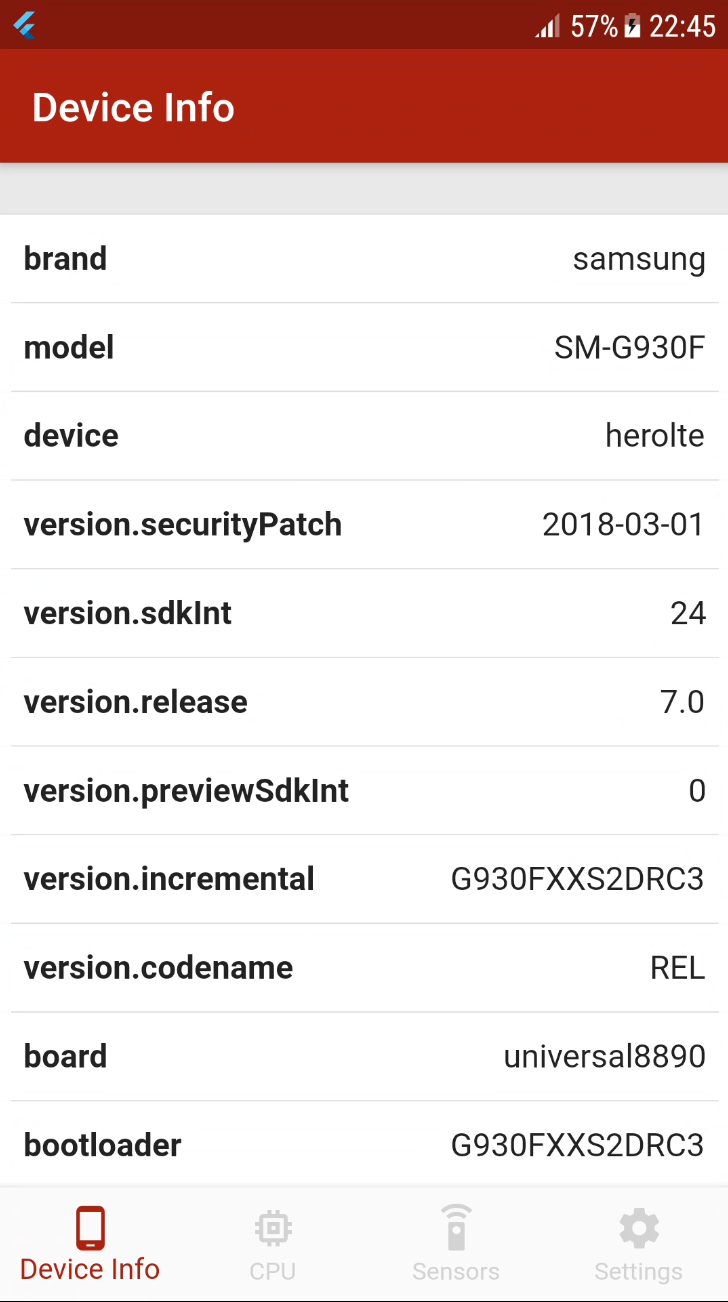
\includegraphics[height=20em]{mobile-device-info}
  \caption{\textit{Device Info} contains various information about the running system.}
\end{figure}

\begin{figure}[H]
  \centering
  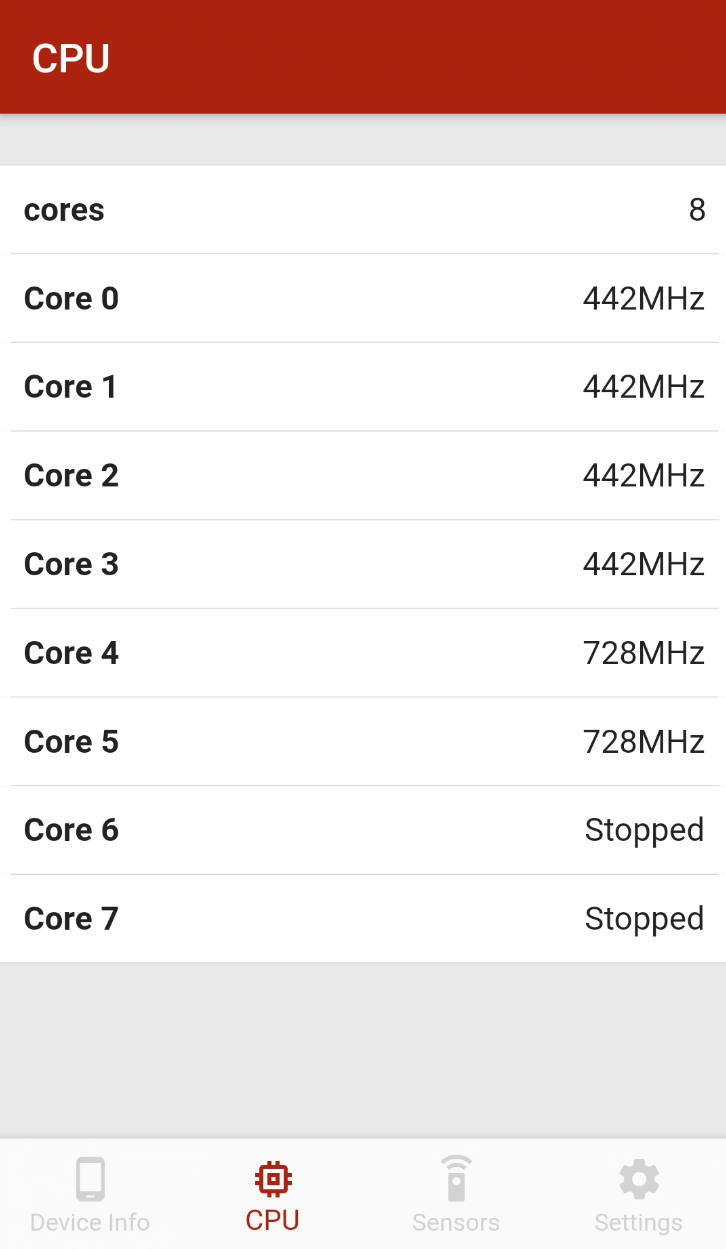
\includegraphics[height=20em]{mobile-cpu}
  \caption{\textit{CPU} shows the amount of cores available and the frequency they are currently
  running at, if they are running at all. This view, however, is only available on \textit{Android}
  due to limitations on retrieval of CPU information on \textit{iOS}.}
\end{figure}

\begin{figure}[H]
  \centering
  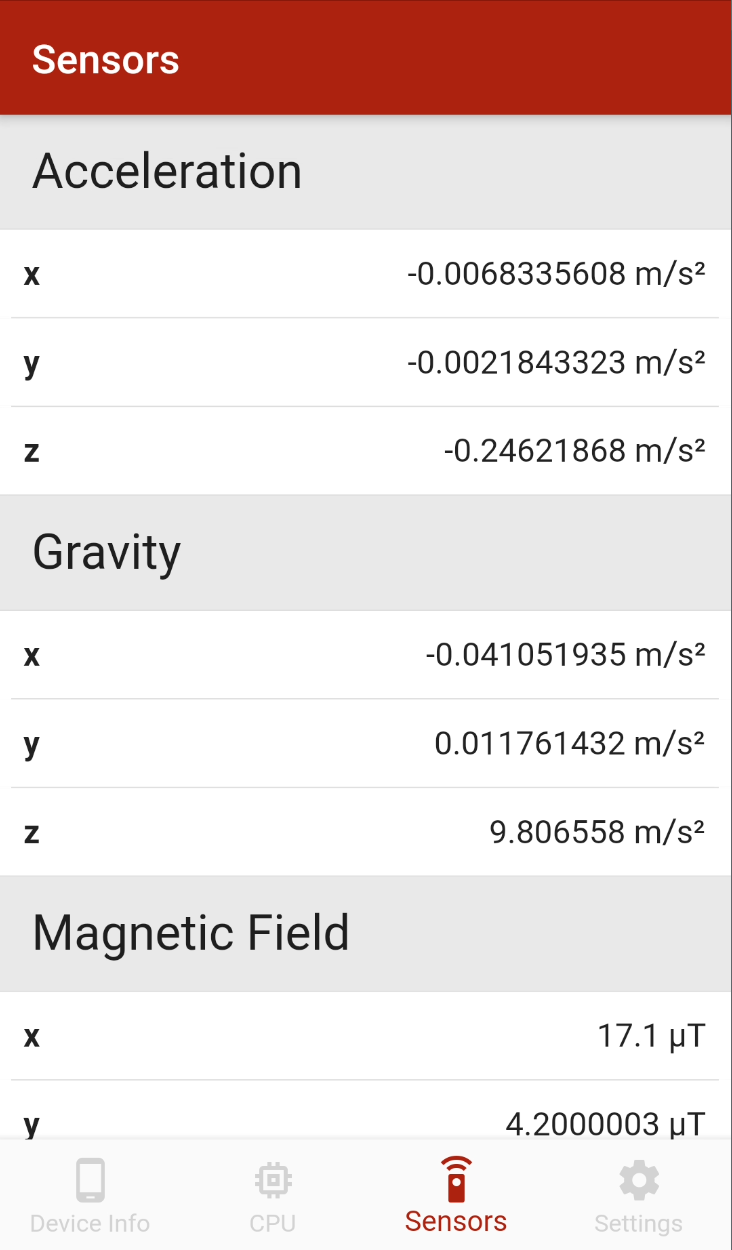
\includegraphics[height=20em]{mobile-sensors}
  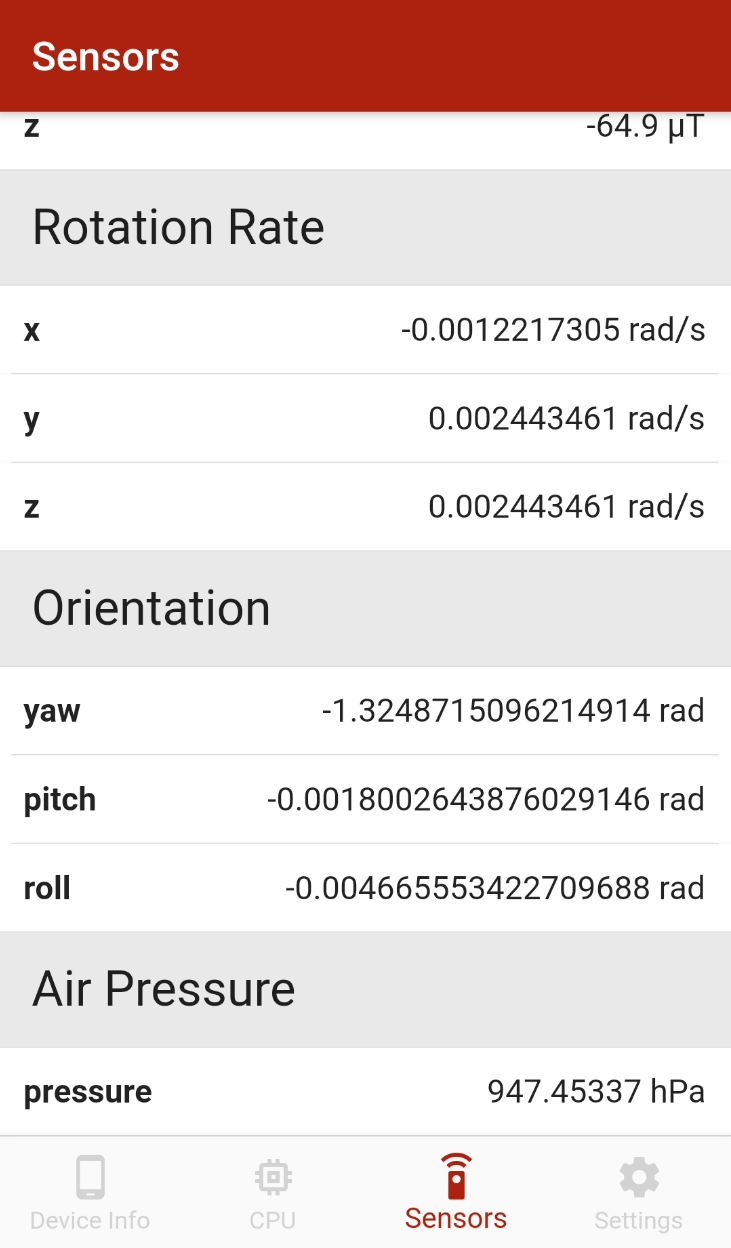
\includegraphics[height=20em]{mobile-sensors-2}
  \caption{\textit{Sensors} lists various sensors on both platforms.}
\end{figure}

\begin{figure}[H]
  \centering
  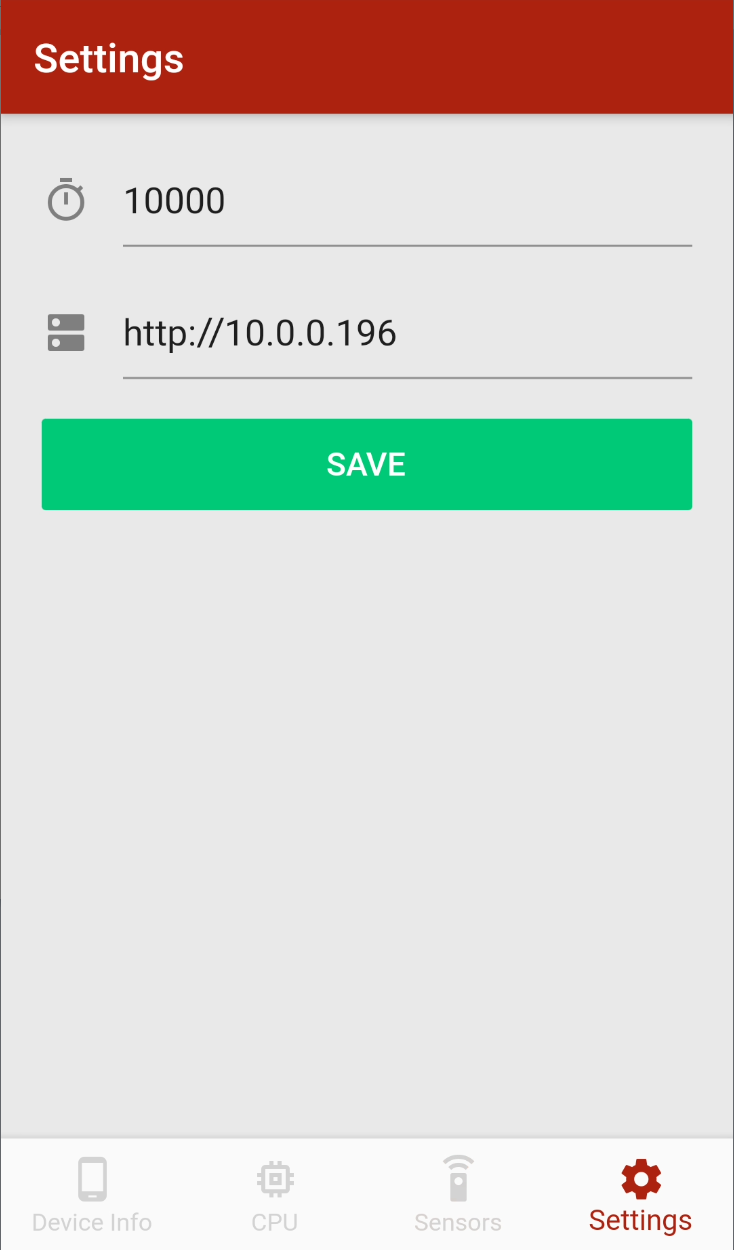
\includegraphics[height=20em]{mobile-settings}
  \caption{\textit{Settings} gives the user the ability to modify the interval of sending data to the
  server and the \textit{URL} where the server is located.}
\end{figure}

The most important part about the application however is sending data to a \textit{Kafka} topic
which then invokes a \textit{serverless function}. To achieve this we wrap all data into categories
and send them to the specific topic in \textit{Kafka} via \textit{JSON}. The task of the
\textit{serverless function} is then to push the data into our \textit{MongoDB} database.

\section{Serverless Stack}

Arguably, the main part of our thesis is the serverless stack hence it's also in the title of the
project. When doing research for our project, thinking about the serverless stack was one of the
first things we did. We came across many different serverless frameworks. \textit{OpenWhisk},
\textit{Fission} and \textit{Kubeless} just to name a few. While all of those seem to have their
benefits, none of them seemed to be as versatile as \textit{OpenFaaS}.

\textit{OpenFaaS} poses itself to have first class support for \textit{Docker Swarm} and being
\textit{Kubernetes} native. The former was particularly interesting for us as this meant that we
could test the framework without having to install any external tool except for  \textit{Docker}.

Running was as simple as cloning the \textit{OpenFaaS} repository, calling \texttt{docker swarm
init} and executing the provided initialisation script. Deploying an actual function is equally
simple. One has the option to either deploy a function from the store through the nicely designed
\textit{OpenFaaS} gateway on port~8080 or with the preferred way, which is using the
\texttt{faas-cli} command line tool.

Deploying a function from the store with it would look as follows:

\begin{lstlisting}[language=bash]
faas store deploy figlet
\end{lstlisting}

Here, \texttt{figlet} is the name of the function in the store.

After gaining a grasp of how the platform works, we decided to put our own spin on it by firstly
modifying the given deploy script to our needs and porting it from \textit{Bash} to \textit{Rust}
for it to be cross platform. The next step then was to write our own configuration file for swarm
deployment, namely \texttt{deploy.yml}. This \textit{YAML} file includes the configuration for
\textit{Kafka}, \textit{Zookeeper}, \textit{MongoDB}, various services that are needed for
\textit{OpenFaaS}, a bunch of gateways for visualisation and the \textit{Kafka-Connector}. All of
these service are \textit{Docker} images and can therefore be easily updated and extended.
\textit{Kafka-Connector} is particularly interesting, because its main purpose is to call a
serverless function on a Kafka topic change. To make a function react to a Kafka topic we can again
use our example store function \texttt{figlet}:

\begin{lstlisting}[language=bash]
faas store deploy figlet --annotation topic="faas-request"
\end{lstlisting}

The deployment aspect is the same as before, therefore the interesting part is the \\
\texttt{-{}-annotation} flag, where \texttt{topic="faas-request"} is the \textit{Kafka} topic the
function is supposed to listen to and act on. We subsequently can look for the result in the logs of
the connector service. \\
While the feature of deploying functions from the store is really nice, it is not suitable for our
use case, as we highly depend on custom functions written by ourselves.

\begin{figure}[H]
  \centering
  \adjincludegraphics[max width=\textwidth]{openfaas-dashboard}
  \caption{Picture of all functions in the \textit{OpenFaaS} dashboard}
\end{figure}

\section{Raspberry Pi}

In order for us to gather data, we decided on using multiple \textit{Raspberry Pis} with different
sensors attached to them. We chose the \textit{Raspberry Pi} because it is backed by a huge
community and because of the vast amount of documentation available for it. Having documentation
available was essential, since we wanted to write the client application for the \textit{Raspberry
Pi} in \textit{Rust}. This way we could validate our \textit{Rust} code by comparing it to example
code written in other programming languages, most commonly \textit{Python} or \textit{C} in the case
of the \textit{Raspberry Pi}.

\subsection{\textit{Rust} on the \textit{Raspberry Pi}}

For our first “Hello, world!” program which would run on the \textit{Raspberry Pi}, we took the
simplest approach at the time. We would write the code on our development machines and synchronise
the code to the \textit{Raspberry Pi} using \texttt{rsync} \cite{rsync} and then compile and run it
via \texttt{ssh}. This worked fine at the time. Once we got to the point where we needed to add more
dependencies for the various sensors and networking, compile times naturally increased to the point
at which it simply wasn't feasible anymore to compile directly using the inadequate processor of the
\textit{Raspberry Pi}. A single build was approaching a compile time of around five minutes on every
single small change to the code, so we had to start looking for alternatives.

\subsection{Cross Compilation}

Soon after we realised that compiling directly on the \textit{Raspberry Pi} was not a good solution,
we had to find a way to cross compile for the \textit{Raspberry Pi}. This was further complicated by
the fact the we were using \textit{macOS} and \textit{Windows}, so none of the pre-compiled cross
compilation \whitelist{toolchains} for \textit{Linux} were an option for us.

We then found the \texttt{cross} \cite{cross} tool, which claimed to automatically install the
corresponding toolchain and then run the cross compilation in a \textit{Docker} container, so this
should have worked on both \textit{macOS} and \textit{Windows}. Right after we installed it using
\texttt{cargo install cross}, we saw that \textit{macOS} and \textit{Windows} support was lacking.
On both platforms, \texttt{cross} tried to simply call \texttt{cargo} directly instead of running in
a \textit{Docker} container. Since this tool still seemed to be the best solution we could find for
our situation and since the tool is open-source, we decided to dig into the source code and add the
missing \textit{macOS} and \textit{Windows} support ourselves.

Getting \texttt{cross} to actually run a \textit{Docker} container on both of our platforms was
quite easy, we only had to add two new definitions for \textit{Rust} toolchains in the source code
of \texttt{cross}, one for \textit{macOS} (\texttt{x86\_64-apple-darwin}) and one for
\textit{Windows} (\texttt{x86\_64-pc-windows-msvc}). The next problem we were facing was that inside
of the \textit{Docker} container, the \texttt{CARGO\_HOME} directory was mounted, and with it, its
\texttt{bin} subdirectory. This meant that the \textit{Docker} container would first look in this
directory instead of the respective toolchain root for the corresponding target's binaries. Since
the binaries in \texttt{CARGO\_HOME/bin} are compiled for the host machine, these previously worked
fine since only \texttt{x86\_64} \textit{Linux} hosts were supported. Now however, it would try
running a \textit{macOS} or \textit{Windows} binary inside of a \textit{Linux} \textit{Docker}
container. This was not as straight-forward to debug as it might seem, since the error message made
it seem as though it was a syntax error in a shell command. Once we found what the problem was, the
next challenge was to actually implement the fix for it. We still had to mount \texttt{CARGO\_HOME},
but exclude its \texttt{bin} subdirectory. Since the contents of \texttt{CARGO\_HOME} can vary
depending on what you have installed, we could not simply mount each subdirectory individually and
exclude \texttt{bin}, so the only way was to use a somewhat hacky workaround.

The whole \texttt{CARGO\_HOME} directory was already mounted using

\begin{lstlisting}[language=Bash]
-v "${CARGO_HOME}:/cargo:Z"
\end{lstlisting}

In order to prevent mounting the \texttt{bin} subdirectory from the host machine, we added

\begin{lstlisting}[language=Bash]
-v /cargo/bin
\end{lstlisting}

This means that technically the \texttt{bin} subdirectory is still mounted, but is overlaid by
another virtual volume which is not bound to a directory on the host, which effectively prevents
non-Linux binaries from being accessible inside the \textit{Docker} container. After this change, we could
finally compile our program on both \textit{macOS} and \textit{Windows}.

\subsection{Sensors}

For the actual collection of data, we of course needed to implement some sensors. The first sensor
we implemented is the widely used \textit{BMP180}, a digital sensor which acts as a combination of a
thermometer and barometer. The \\ \textit{BMP180} communicates over the \textit{I\textsuperscript{2}C}
bus. \textit{I\textsuperscript{2}C} is supported natively by most \textit{Linux} distributions,
consequentially also by the \textit{Raspbian} operating system running on the \textit{Raspberry Pi}.
We quickly found a \textit{Rust} library called \texttt{i2cdev}, which provides idiomatic wrapper functions
to interface with the \textit{Linux} \textit{I\textsuperscript{2}C} interface. Another library
called \texttt{i2cdev\_bmp180} then gave us an API for performing temperature and air pressure
measurements.

The second sensor we wanted to implement is the \textit{AM2320}, a digital temperature and humidity
sensor. The \textit{AM2320} also communicates over the \textit{I\textsuperscript{2}C} bus, which
means we could use a \textit{Rust} library fittingly called \textit{am2320}, which also is based on the
\textit{i2cdev} library, to produce temperature and humidity measurements. We also contributed some
improvements (see \url{https://github.com/gferon/am2320.rs/pull/1}) to this library.

The last sensor we implemented is a simple analogue photoresistor acting as a luminosity sensor. Due
to the fact that the \textit{Raspberry Pi} does not have any analogue \textit{GPIO} pins, we had to
resort to using an analogue-to-digital converter. To simplify the implementation of such a
converter, we chose the \textit{ADS1115}, which like the \textit{BMP180} and \textit{AM2320}
communicates over the \textit{I\textsuperscript{2}C} bus. With the \texttt{ads1x1x} library, we
could read the analogue photoresistor's voltage. By knowing this voltage, we can then
approximate the luminosity.

\begin{figure}[H]
  \centering
  \adjincludegraphics[max width=\textwidth]{wiring}
  \caption{Wiring diagram of sensors connected to a \textit{Raspberry Pi}}
  \label{fig:raspberry-wiring}
\end{figure}

In \autoref{fig:raspberry-wiring} we can see how the sensors are connected to the \textit{Raspberry
Pi}. The orange and red wires signify the 3.3V and 5V power supply lanes, respectively. The black
wire is the ground connection, and blue and violet are the two wires (receive/transmit) for the
\textit{I\textsuperscript{2}C} bus. From top to bottom, you can see the photoresistor connected to
the analogue-to-digital converter (ADC), followed by the \textit{BMP180} and the \textit{AM2320}. It
is easy to see that all sensors share the same \textit{I\textsuperscript{2}C} bus by looking at the
diagram.

\subsection{Serverless UI}

Another instrumental part of the project is the UI. Without any form of visualisation our whole data
gathering process would not be of much use. For this reason we decided early on what kind of front
end web development stack we would use. Since both us are familiar with \textit{React} - a
\textit{JavaScript} framework famous for revolutionising the use of the \textit{virtual DOM}
to render \textit{UI} elements and to update \textit{UI} elements reactively on
UI change - we decided on using \textit{MarkoJS}.

\subsubsection{MarkoJS}

\textit{MarkoJS} shares many of the same benefits as \textit{React} with some added flexibility like
\textit{concise HTML syntax} which makes the whole \textit{markup} more readable and easier to
write. It also has the ability to use conventional control flow structures like \textit{if} or
\textit{for} directly in the \textit{markup}.

\subsubsection{Babel}

However \textit{MarkoJS} is most and foremost a \textit{JavaScript} framework and due to the nature
of the before mentioned features, \textit{transpiling} is inevitable. \textit{Transpiling} means to
transform modern possibly unsupported \textit{JavaScript} into valid \textit{ECMAScript 5} compliant
code that any browser can understand. For this process we currently use the industry standard
technology \textit{Babel}. With \textit{Babel} \textit{transpiling} is rather easy. All necessary
definitions are in a \textit{webpack.config.babel.js} file which brings us to the next essential
tool \textit{Webpack}.

\subsubsection{Webpack}

“Webpack is a module bundler. Its main purpose is to bundle JavaScript files for usage in a browser,
yet it is also capable of transforming, bundling, or packaging just about any resource or asset.”

With that being said \textit{Webpack} can to some extend be considered as the main part of the whole
\textit{front end stack} as it is responsible for orchestrating \textit{transpiling} of
\textit{MarkoJS} files. It is also responsible for providing \textit{Webpack Dev Server}, a server
that reloads on file change. Furthermore \textit{Webpack} runs all files through certain
optimisation plugins on release build, which can bring down the size of the \textit{code bundle}
quite considerably. \textit{Webpack} is also able to transform \textit{SASS} into \textit{CSS}.

\subsubsection{SASS}

\textit{SASS} is a superset of \textit{CSS} with many additional features like variables, functions,
nesting and exporting / importing files. We make heavy use of those features to structure and
modularise our \textit{CSS} code.

\subsection{UI}

The \textit{UI} itself uses a basic layout where all sensor devices registered in the database are
listed on the side in a so called \textit{sidebar}. The user then can click on each individual
device to open a view with detailed graphs of sensor data of that device. The categories of graphs
are different according to device group. For example \textit{IoT devices} will have different
sensors compared to phones. After a device is selected, the user can then specify the begin and end
time interval according to which sensor data of that device will be filtered and the amount of time
slices. By default the timespan is limited to 24 hours and to 24 time slices. A time slice in our
case is a division of a time interval into equally long time units. To get a single value per time
slice we average all sensor values of a specific sensor between two time slices. Those single values
will then be displayed in the graphs.


  \chapter{Results}
\label{sec:results}

\section{Benchmarks}

For our test setup, we deployed our stack on an \textit{Intel NUC}, which is a fairly inexpensive
mini PC. With the following benchmarks, we want to show what such an affordable machine is capable
of when coupled with other cheap IoT devices, e.g. a Raspberry Pi.

\begin{table}[H]
  \centering
  \begin{tabular}{|l|l|l|r|}
    \hline
    Name                     & Model              & Processor                                                                             & Memory              \\ \hline
    \whitelist{Intel NUC}    & \whitelist{8I5BEH} & \whitelist{Intel Core i5-8259U} @ \SI{2.30}{\giga\hertz}                              & \SI{16}{\giga\byte} \\ \hline
    \whitelist{Raspberry Pi} & 3 B+               & \whitelist{Broadcom BCM2837B0, 64-bit SoC} @ \SI{1.4}{\giga\hertz}                    & \SI{1}{\giga\byte}  \\ \hline
    Desktop PC               & –                  & \whitelist{Intel Core i9-7900X} @ \SI{4.7}{\giga\hertz}                               & \SI{64}{\giga\byte} \\ \hline
  \end{tabular}
  \caption{Hardware used for Benchmark}
  \label{tab:benchmark-hardware}
\end{table}

The specific hardware we used for benchmarking is listed in \autoref{tab:benchmark-hardware} above.
The desktop PC and the \textit{NUC} were both connected via \whitelist{ethernet} to a \SI{1}{\giga\bit} network
switch. The \textit{Raspberry Pi} was connected via WiFi to an access point connected to the same
switch. \autoref{tab:benchmark-network-speed} shows the link speed between the hardware components
as tested with \texttt{iperf3} \cite{iperf}.

\begin{table}[H]
  \centering
  \begin{tabular}{|l|r|}
    \hline
    Connection                                  & Speed                          \\ \hline
    \textit{NUC} $\leftrightarrow$ Desktop PC   & \SI{940}{\mega\bit\per\second} \\ \hline
    \textit{NUC} $\leftrightarrow$ Raspberry Pi & \SI{55}{\mega\bit\per\second}  \\ \hline
  \end{tabular}
  \caption{Link speed between Hardware Components}
  \label{tab:benchmark-network-speed}
\end{table}


\begin{table}[H]
  \centering
  \begin{tabular}{|r|r|}
    \hline
    Number of Sensors & Messages per Second \\ \hline
                    1 &                7.55 \\ \hline
                    8 &               49.20 \\ \hline
  \end{tabular}
  \caption{Benchmark for Messages per Second from a Raspberry Pi to a \whitelist{NUC}}
  \label{tab:benchmark-nuc-raspberry-pi}
\end{table}

In \autoref{tab:benchmark-nuc-raspberry-pi}, we see the benchmark data for the \texttt{log-data}
function. For this benchmark, we set the \textit{Raspberry Pi} to not use any delay between
measurements instead of the usual measurement interval of \SI{15}{\second}. We also disabled the
\texttt{CPU Load Aggregate} measurement, since this has an inherent delay of \SI{1}{\second} due to
the fact that it calculates the load average for a given duration. The \textit{Raspberry Pi}
application collects the data for all sensors in each iteration, which means that we can actually
get much more throughput with eight sensors than with a single sensor. Thus, we can further
conclude that the time to produce a measurement is negligible compared to the network latency.

In order to test this theory, we decided to use parallel \texttt{curl} requests from a more
powerful computer to test the limit of the \textit{NUC}.

\begin{table}[H]
  \centering
  \begin{tabular}{|r|r|}
    \hline
    Number of concurrent Requests & Messages per Second \\ \hline
                                1 &                61.2 \\ \hline
                               10 &               239.0 \\ \hline
                               20 &               322.4 \\ \hline
                               50 &               379.5 \\ \hline
  \end{tabular}
  \caption{Benchmark for Messages per Second from a Desktop PC to a \whitelist{NUC}}
  \label{tab:benchmark-nuc-curl}
\end{table}

Each \texttt{curl} request in \autoref{tab:benchmark-nuc-curl} contains a single sensor record which
corresponds to the case in \autoref{tab:benchmark-nuc-raspberry-pi} with a single sensor. By looking
at this data, we can see when only sending data for a single sensor, the \textit{Raspberry Pi} is
clearly the bottleneck, not the \textit{NUC}. It is safe to assume that the \textit{NUC} is able to
handle approximately 400~requests per second.

With this assumption that a \textit{NUC} can handle 400~requests per second, we can deduce that with
our test setup, we are able to process streams from between

$\frac{400}{7.55} \times 1 \approx 53$

and

$\frac{400}{49.20} \times 8 \approx 65$

sensors.

This being a synthetic benchmark, it is likely that in a real world scenario, where sensor data is
sent only every \textit{x} seconds, the number of supported sensors is actually in the~100s instead
of only in the~10s.


  \section{Progress}

Our task is to do \textit{IoT data analytics with serverless computing}, therefore as a first step we started out by thinking about the underlying infrastructure. We decided on using Apache Kafka for streaming,  \textit{MongoDB} as our database and \textit{OpenFaaS} as the serverless platform. \\
The decision to use \textit{OpenFaaS} was made because of its ease to deploy a stack of services using \textit{Docker Swarm}.
While doing research we came across many different serverless frameworks. \textit{OpenWhisk}, \textit{Fission} and \textit{Kubeless} just to name a few. While all of those seem to have their benefits, none of them seemed to be as versatile as \textit{OpenFaaS}. \textit{OpenFaaS} poses itself to have first class support for \textit{Docker Swarm} and being \textit{Kubernetes} native. The former was particularly interesting for us as this meant that we could test the framework without having to install any external tool except for  \textit{Docker}. Running was as simple as cloning the \textit{OpenFaaS} repository, calling \texttt{docker swarm init} and executing the provided initialization script. Deploying an actual function is equally as simple. One has the option to either deploy a function from the store through the nicely designed  \textit{OpenFaaS} gateway on port 8080 or with the prefered way, which is using the \textit{faas-cli}. Deploying a function from the store with it would look as follows

\begin{lstlisting}[language=bash]
  $ faas store deploy figlet
\end{lstlisting}

where \texttt{figlet} is the name of the function in the store.\\
\\
After gaining a grasp of how the platform works, we decided to put our own spin on it by firstly modifying the given deploy script to our needs and porting it from \textit{Bash} to \textit{Rust} for it to be cross platform. The next step then was to write our own configuration file for swarm deployment, namely \texttt{deploy.yml}. This \textit{YAML} file includes the configuration for \textit{Kafka}, \textit{Zookeeper}, \textit{MongoDB}, various services that are needed for \textit{OpenFaaS}, a bunch of gateways for visualisation and the \textit{Kafka-Connector}. The latter is particularly interesting, because its main purpose is to call a serverless function on a Kafka topic change. To make a function react to a Kafka topic we can again use our example store function \texttt{figlet}

\begin{lstlisting}[language=bash]
  $ faas store deploy figlet --annotation topic="faas-request"
\end{lstlisting}

The deployment aspect is the same as before therefore the interesting part is the \texttt{-{}-annotation} flag, where \texttt{topic="faas-request"} is the \textit{Kafka} topic the function is supposed to listen to and act on. We subsequently can look for the result in the logs of the connector service. \\
While our technology stack for the most part was nice to work with, we still had our fair share of problems. The most significant so far was in relation to our \textit{MongoDB} database. \textit{MongoDB's} API design is confusing to say the least. Questionable deprecation choices and multiple connect interfaces are the most rampant examples. Unfortunately those were not the only problems in that regard we ran into. Connecting through a node instance natively on the system would work fine, however connecting through a deployed function in \textit{OpenFaaS} was not possible. After applying various fixes the function was finally able to connect. \\
The next challenge will be to post to the database through the \textit{Kafka-Connector}. When that is done we can finally focus on gathering data from IoT devices.

  \subsection{Mobile Application}

Another one of our tasks was to create a mobile application that fetches data from the respective
device and sends data to a \textit{Kafka} topic which subsequently invokes a \textit{serverless
function} to finally persist that data in a \textit{MongoDB} database. To approach this topic we
first did some research on current possibilities on creating cross platform mobile applications and
the general feasibility of the task at hand. It became quite apparent early on that the desired
design for the application is not possible on \textit{iOS}.

The idea for the design of the app is actually rather simple. Get data from the device, no matter if
the application is in foreground, background or the screen is off and the device subsequently
basically being in standby. On \textit{Android} this can be realised easily with a so called
\textit{ForegroundService}. On \textit{iOS} going for the same approach is difficult because of its
restrictions on background tasks. While obviously applications like music players can run in the
background on that platform, achieving the same for a highly battery intensive app like the one we
are developing, is more or less impossible.

Mainly for that reason we actually chose to go for a cross platform mobile application, so we can
have a fully supported \textit{Android} version and also an \textit{iOS} version with limited
functionality.

Finding the ideal tool for our job of creating an application supporting both \textit{iOS} and
\textit{Android} seemed at first pretty easy. We chose to use \textit{React Native} as we both
already have experience with \textit{React} itself and the approach to \textit{UI design} seemed
equally elegant.

Getting started with \textit{React Native} was rather fast and effortless, the same however could
not be said anymore once we progressed further with the project. At first things were looking good
as the UI did properly respond to data from sensors / CPU but as we added more and more data for
display, the UI got more and more sluggish to the point that it could not be considered usable
anymore. Unfortunately this was not the only problem.

By nature the application relies heavily on \textit{native code}. The main culprit for this is the
\textit{ForegroundService} on \textit{Android}. \textit{React Native} has a so called
\textit{bridge} for communication between \textit{native code} and the \textit{UI}. Our application
uses that bridge heavily for retrieving information from the service and also to push data to the
service.

Once we fully implemented the settings view and were basically finished with the application, the
app started to crash constantly on \textit{Android}. Unfortunately the tooling of \textit{React
Native} really does not help with debugging fatal crashes. So we had to make a conscious decision
whether we want to continue with \textit{React Native} or start over with something else entirely.

In the end we concluded to search for other frameworks as we deemed \textit{React Native} as
incompatible for our task. We then decided on using \textit{Flutter}. \textit{Flutter} is a modern
cross platform mobile application framework by \textit{Google}. \textit{Flutter} compiles down to
native code and therefore should have a performance advantage compared to \textit{React Native}.

As with any new programming language, \textit{Dart} - the language behind \textit{Flutter} - took
some time to get used to and be productive with. After a while however the process of designing
\textit{UIs} with \textit{Flutter} and writing logic was rather seamless. Fortunately the native
part of the \textit{React Native} application could almost fully be reused for the \textit{Flutter}
version of the app. The surprisingly easy to use \textit{bridge} between native code and
\textit{Dart} in \textit{Flutter} made the transition from \textit{React Native} regarding native
code on \textit{Android} painless.

One of the reason we first chose to use \textit{React Native} was the extensive community support.
Getting sensor data from almost all supported sensors on \textit{iOS} was as simple as including a
package. The same cannot be said about \textit{Flutter}. For that reason we also had to write some
native code for \textit{iOS} which splits the code base further.

The finished application now contains four Views:

\begin{figure}[H]
  \centering
  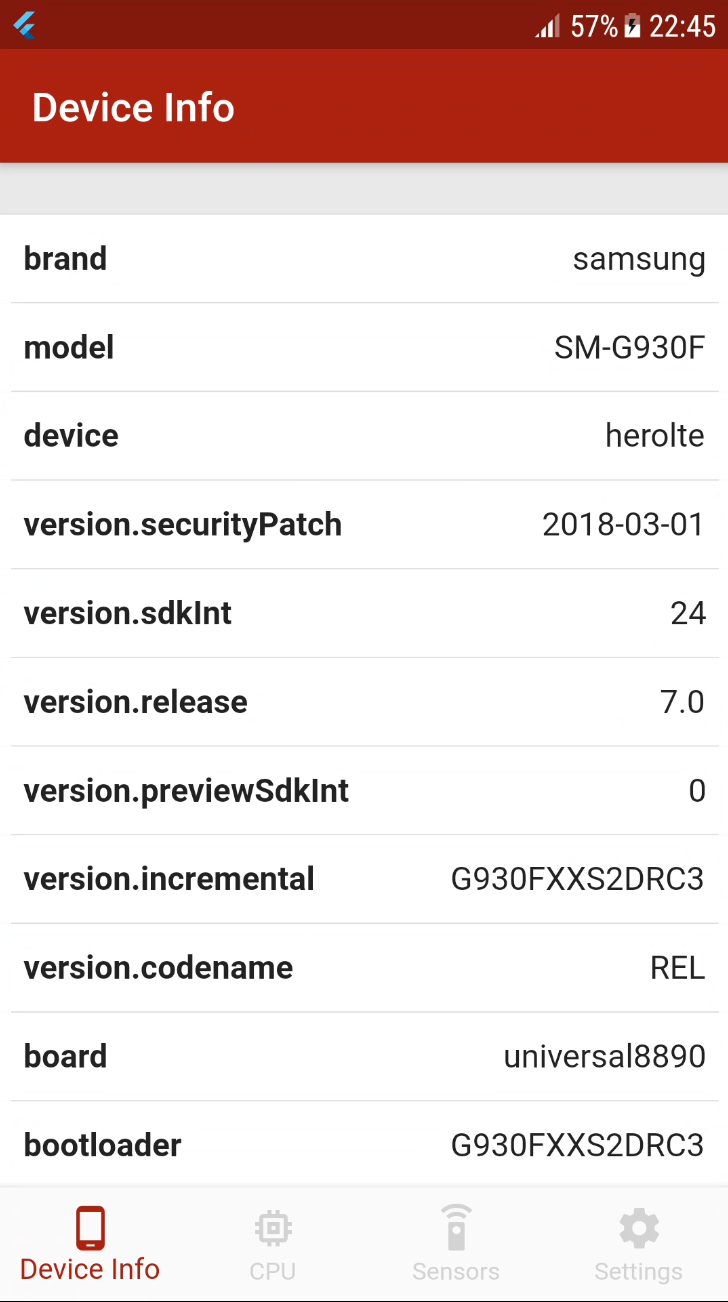
\includegraphics[height=20em]{mobile-device-info}
  \caption{\textit{Device Info} contains various information about the running system.}
\end{figure}

\begin{figure}[H]
  \centering
  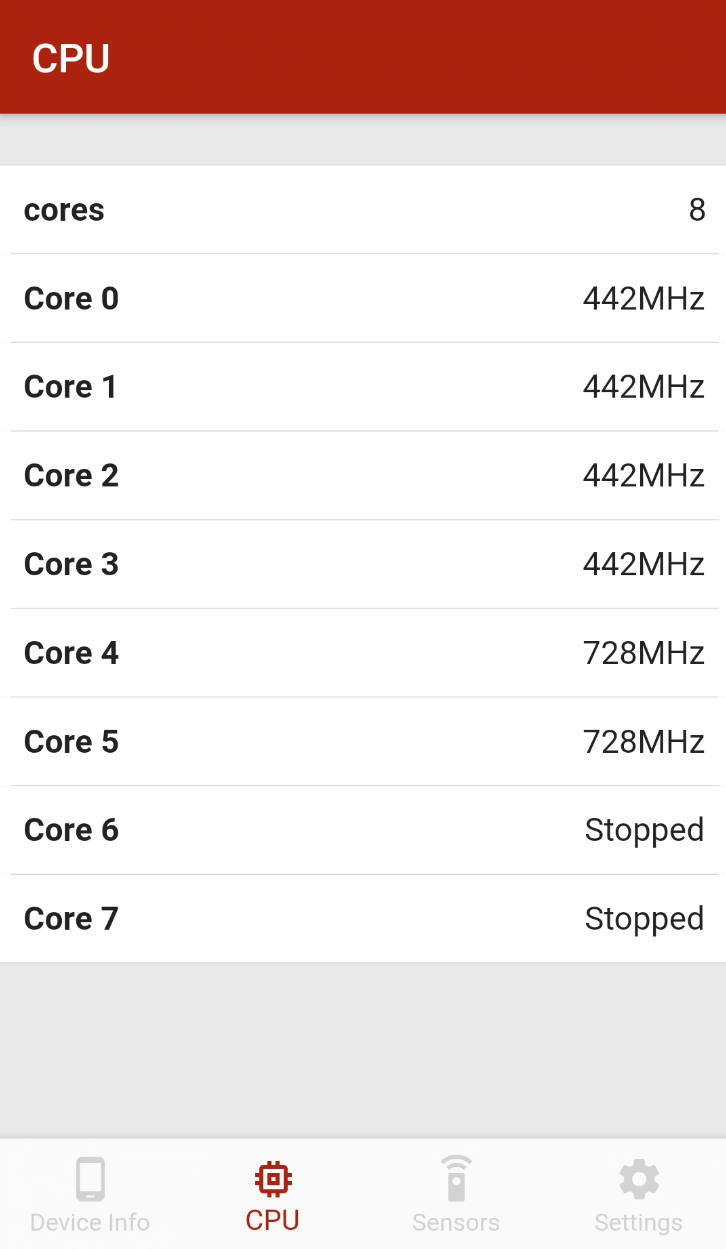
\includegraphics[height=20em]{mobile-cpu}
  \caption{\textit{CPU} shows the amount of cores available and the frequency they are currently
  running at, if they are running at all. This view, however, is only available on \textit{Android}
  due to limitations on retrieval of CPU information on \textit{iOS}.}
\end{figure}

\begin{figure}[H]
  \centering
  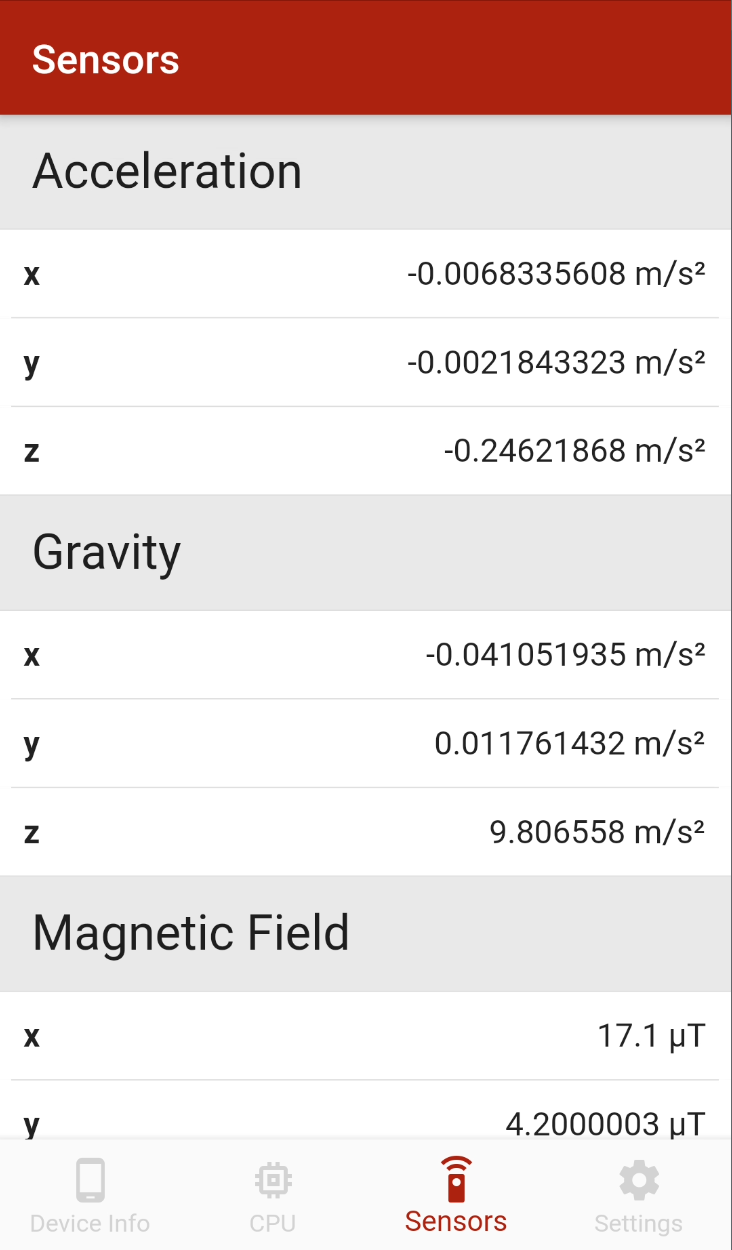
\includegraphics[height=20em]{mobile-sensors}
  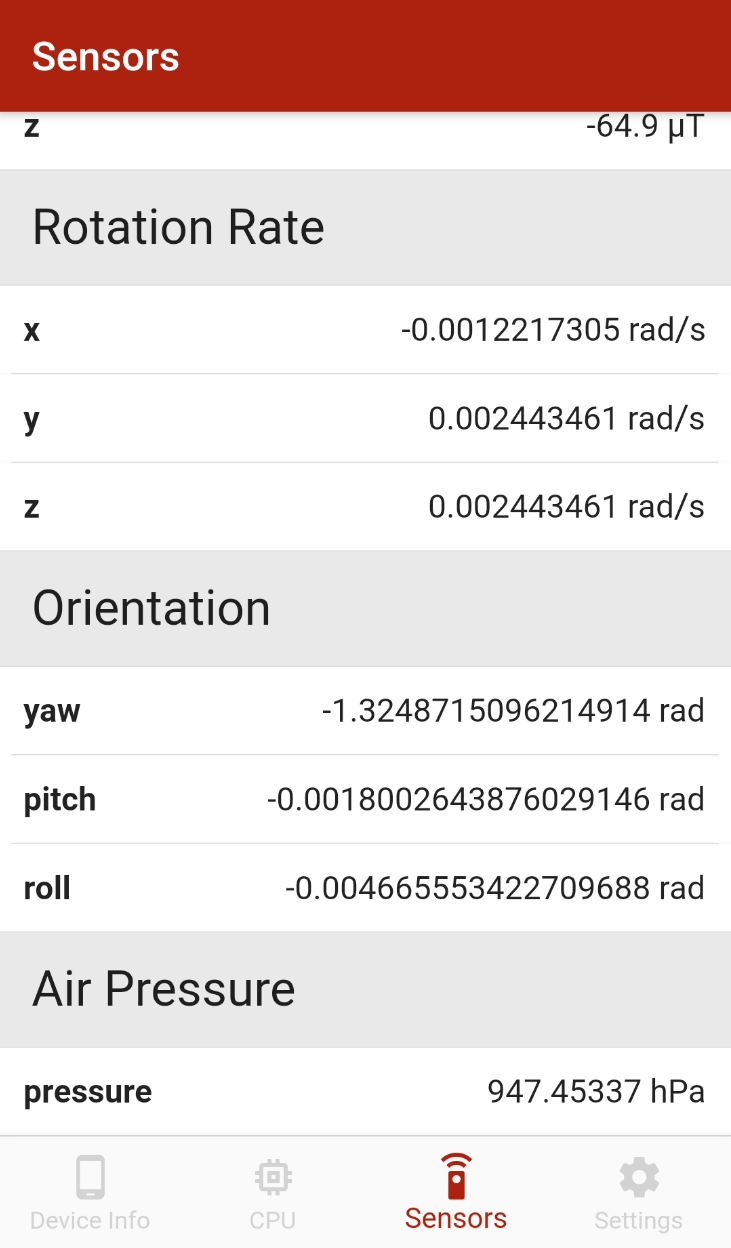
\includegraphics[height=20em]{mobile-sensors-2}
  \caption{\textit{Sensors} lists various sensors on both platforms.}
\end{figure}

\begin{figure}[H]
  \centering
  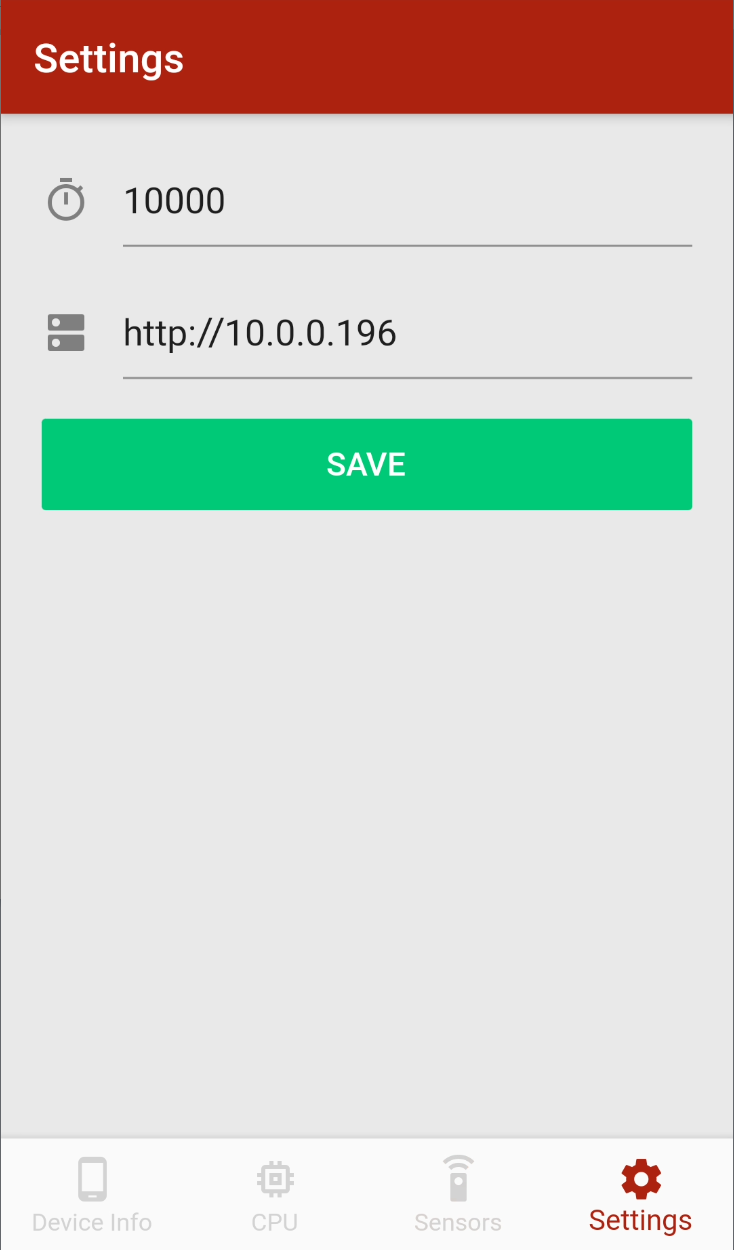
\includegraphics[height=20em]{mobile-settings}
  \caption{\textit{Settings} gives the user the ability to modify the interval of sending data to the
  server and the \textit{URL} where the server is located.}
\end{figure}

The most important part about the application however is sending data to a \textit{Kafka} topic
which then invokes a \textit{serverless function}. To achieve this we wrap all data into categories
and send them to the specific topic in \textit{Kafka} via \textit{JSON}. The task of the
\textit{serverless function} is then to push the data into our \textit{MongoDB} database.

  \section{Serverless Stack}

Arguably, the main part of our thesis is the serverless stack hence it's also in the title of the
project. When doing research for our project, thinking about the serverless stack was one of the
first things we did. We came across many different serverless frameworks. \textit{OpenWhisk},
\textit{Fission} and \textit{Kubeless} just to name a few. While all of those seem to have their
benefits, none of them seemed to be as versatile as \textit{OpenFaaS}.

\textit{OpenFaaS} poses itself to have first class support for \textit{Docker Swarm} and being
\textit{Kubernetes} native. The former was particularly interesting for us as this meant that we
could test the framework without having to install any external tool except for  \textit{Docker}.

Running was as simple as cloning the \textit{OpenFaaS} repository, calling \texttt{docker swarm
init} and executing the provided initialisation script. Deploying an actual function is equally
simple. One has the option to either deploy a function from the store through the nicely designed
\textit{OpenFaaS} gateway on port~8080 or with the preferred way, which is using the
\texttt{faas-cli} command line tool.

Deploying a function from the store with it would look as follows:

\begin{lstlisting}[language=bash]
faas store deploy figlet
\end{lstlisting}

Here, \texttt{figlet} is the name of the function in the store.

After gaining a grasp of how the platform works, we decided to put our own spin on it by firstly
modifying the given deploy script to our needs and porting it from \textit{Bash} to \textit{Rust}
for it to be cross platform. The next step then was to write our own configuration file for swarm
deployment, namely \texttt{deploy.yml}. This \textit{YAML} file includes the configuration for
\textit{Kafka}, \textit{Zookeeper}, \textit{MongoDB}, various services that are needed for
\textit{OpenFaaS}, a bunch of gateways for visualisation and the \textit{Kafka-Connector}. All of
these service are \textit{Docker} images and can therefore be easily updated and extended.
\textit{Kafka-Connector} is particularly interesting, because its main purpose is to call a
serverless function on a Kafka topic change. To make a function react to a Kafka topic we can again
use our example store function \texttt{figlet}:

\begin{lstlisting}[language=bash]
faas store deploy figlet --annotation topic="faas-request"
\end{lstlisting}

The deployment aspect is the same as before, therefore the interesting part is the \\
\texttt{-{}-annotation} flag, where \texttt{topic="faas-request"} is the \textit{Kafka} topic the
function is supposed to listen to and act on. We subsequently can look for the result in the logs of
the connector service. \\
While the feature of deploying functions from the store is really nice, it is not suitable for our
use case, as we highly depend on custom functions written by ourselves.

\begin{figure}[H]
  \centering
  \adjincludegraphics[max width=\textwidth]{openfaas-dashboard}
  \caption{Picture of all functions in the \textit{OpenFaaS} dashboard}
\end{figure}

  \section{Raspberry Pi}

In order for us to gather data, we decided on using multiple \textit{Raspberry Pis} with different
sensors attached to them. We chose the \textit{Raspberry Pi} because it is backed by a huge
community and because of the vast amount of documentation available for it. Having documentation
available was essential, since we wanted to write the client application for the \textit{Raspberry
Pi} in \textit{Rust}. This way we could validate our \textit{Rust} code by comparing it to example
code written in other programming languages, most commonly \textit{Python} or \textit{C} in the case
of the \textit{Raspberry Pi}.

\subsection{\textit{Rust} on the \textit{Raspberry Pi}}

For our first “Hello, world!” program which would run on the \textit{Raspberry Pi}, we took the
simplest approach at the time. We would write the code on our development machines and synchronise
the code to the \textit{Raspberry Pi} using \texttt{rsync} \cite{rsync} and then compile and run it
via \texttt{ssh}. This worked fine at the time. Once we got to the point where we needed to add more
dependencies for the various sensors and networking, compile times naturally increased to the point
at which it simply wasn't feasible anymore to compile directly using the inadequate processor of the
\textit{Raspberry Pi}. A single build was approaching a compile time of around five minutes on every
single small change to the code, so we had to start looking for alternatives.

\subsection{Cross Compilation}

Soon after we realised that compiling directly on the \textit{Raspberry Pi} was not a good solution,
we had to find a way to cross compile for the \textit{Raspberry Pi}. This was further complicated by
the fact the we were using \textit{macOS} and \textit{Windows}, so none of the pre-compiled cross
compilation \whitelist{toolchains} for \textit{Linux} were an option for us.

We then found the \texttt{cross} \cite{cross} tool, which claimed to automatically install the
corresponding toolchain and then run the cross compilation in a \textit{Docker} container, so this
should have worked on both \textit{macOS} and \textit{Windows}. Right after we installed it using
\texttt{cargo install cross}, we saw that \textit{macOS} and \textit{Windows} support was lacking.
On both platforms, \texttt{cross} tried to simply call \texttt{cargo} directly instead of running in
a \textit{Docker} container. Since this tool still seemed to be the best solution we could find for
our situation and since the tool is open-source, we decided to dig into the source code and add the
missing \textit{macOS} and \textit{Windows} support ourselves.

Getting \texttt{cross} to actually run a \textit{Docker} container on both of our platforms was
quite easy, we only had to add two new definitions for \textit{Rust} toolchains in the source code
of \texttt{cross}, one for \textit{macOS} (\texttt{x86\_64-apple-darwin}) and one for
\textit{Windows} (\texttt{x86\_64-pc-windows-msvc}). The next problem we were facing was that inside
of the \textit{Docker} container, the \texttt{CARGO\_HOME} directory was mounted, and with it, its
\texttt{bin} subdirectory. This meant that the \textit{Docker} container would first look in this
directory instead of the respective toolchain root for the corresponding target's binaries. Since
the binaries in \texttt{CARGO\_HOME/bin} are compiled for the host machine, these previously worked
fine since only \texttt{x86\_64} \textit{Linux} hosts were supported. Now however, it would try
running a \textit{macOS} or \textit{Windows} binary inside of a \textit{Linux} \textit{Docker}
container. This was not as straight-forward to debug as it might seem, since the error message made
it seem as though it was a syntax error in a shell command. Once we found what the problem was, the
next challenge was to actually implement the fix for it. We still had to mount \texttt{CARGO\_HOME},
but exclude its \texttt{bin} subdirectory. Since the contents of \texttt{CARGO\_HOME} can vary
depending on what you have installed, we could not simply mount each subdirectory individually and
exclude \texttt{bin}, so the only way was to use a somewhat hacky workaround.

The whole \texttt{CARGO\_HOME} directory was already mounted using

\begin{lstlisting}[language=Bash]
-v "${CARGO_HOME}:/cargo:Z"
\end{lstlisting}

In order to prevent mounting the \texttt{bin} subdirectory from the host machine, we added

\begin{lstlisting}[language=Bash]
-v /cargo/bin
\end{lstlisting}

This means that technically the \texttt{bin} subdirectory is still mounted, but is overlaid by
another virtual volume which is not bound to a directory on the host, which effectively prevents
non-Linux binaries from being accessible inside the \textit{Docker} container. After this change, we could
finally compile our program on both \textit{macOS} and \textit{Windows}.

\subsection{Sensors}

For the actual collection of data, we of course needed to implement some sensors. The first sensor
we implemented is the widely used \textit{BMP180}, a digital sensor which acts as a combination of a
thermometer and barometer. The \\ \textit{BMP180} communicates over the \textit{I\textsuperscript{2}C}
bus. \textit{I\textsuperscript{2}C} is supported natively by most \textit{Linux} distributions,
consequentially also by the \textit{Raspbian} operating system running on the \textit{Raspberry Pi}.
We quickly found a \textit{Rust} library called \texttt{i2cdev}, which provides idiomatic wrapper functions
to interface with the \textit{Linux} \textit{I\textsuperscript{2}C} interface. Another library
called \texttt{i2cdev\_bmp180} then gave us an API for performing temperature and air pressure
measurements.

The second sensor we wanted to implement is the \textit{AM2320}, a digital temperature and humidity
sensor. The \textit{AM2320} also communicates over the \textit{I\textsuperscript{2}C} bus, which
means we could use a \textit{Rust} library fittingly called \textit{am2320}, which also is based on the
\textit{i2cdev} library, to produce temperature and humidity measurements. We also contributed some
improvements (see \url{https://github.com/gferon/am2320.rs/pull/1}) to this library.

The last sensor we implemented is a simple analogue photoresistor acting as a luminosity sensor. Due
to the fact that the \textit{Raspberry Pi} does not have any analogue \textit{GPIO} pins, we had to
resort to using an analogue-to-digital converter. To simplify the implementation of such a
converter, we chose the \textit{ADS1115}, which like the \textit{BMP180} and \textit{AM2320}
communicates over the \textit{I\textsuperscript{2}C} bus. With the \texttt{ads1x1x} library, we
could read the analogue photoresistor's voltage. By knowing this voltage, we can then
approximate the luminosity.

\begin{figure}[H]
  \centering
  \adjincludegraphics[max width=\textwidth]{wiring}
  \caption{Wiring diagram of sensors connected to a \textit{Raspberry Pi}}
  \label{fig:raspberry-wiring}
\end{figure}

In \autoref{fig:raspberry-wiring} we can see how the sensors are connected to the \textit{Raspberry
Pi}. The orange and red wires signify the 3.3V and 5V power supply lanes, respectively. The black
wire is the ground connection, and blue and violet are the two wires (receive/transmit) for the
\textit{I\textsuperscript{2}C} bus. From top to bottom, you can see the photoresistor connected to
the analogue-to-digital converter (ADC), followed by the \textit{BMP180} and the \textit{AM2320}. It
is easy to see that all sensors share the same \textit{I\textsuperscript{2}C} bus by looking at the
diagram.

  \subsection{Serverless UI}

Another instrumental part of the project is the UI. Without any form of visualisation our whole data
gathering process would not be of much use. For this reason we decided early on what kind of front
end web development stack we would use. Since both us are familiar with \textit{React} - a
\textit{JavaScript} framework famous for revolutionising the use of the \textit{virtual DOM}
to render \textit{UI} elements and to update \textit{UI} elements reactively on
UI change - we decided on using \textit{MarkoJS}.

\subsubsection{MarkoJS}

\textit{MarkoJS} shares many of the same benefits as \textit{React} with some added flexibility like
\textit{concise HTML syntax} which makes the whole \textit{markup} more readable and easier to
write. It also has the ability to use conventional control flow structures like \textit{if} or
\textit{for} directly in the \textit{markup}.

\subsubsection{Babel}

However \textit{MarkoJS} is most and foremost a \textit{JavaScript} framework and due to the nature
of the before mentioned features, \textit{transpiling} is inevitable. \textit{Transpiling} means to
transform modern possibly unsupported \textit{JavaScript} into valid \textit{ECMAScript 5} compliant
code that any browser can understand. For this process we currently use the industry standard
technology \textit{Babel}. With \textit{Babel} \textit{transpiling} is rather easy. All necessary
definitions are in a \textit{webpack.config.babel.js} file which brings us to the next essential
tool \textit{Webpack}.

\subsubsection{Webpack}

“Webpack is a module bundler. Its main purpose is to bundle JavaScript files for usage in a browser,
yet it is also capable of transforming, bundling, or packaging just about any resource or asset.”

With that being said \textit{Webpack} can to some extend be considered as the main part of the whole
\textit{front end stack} as it is responsible for orchestrating \textit{transpiling} of
\textit{MarkoJS} files. It is also responsible for providing \textit{Webpack Dev Server}, a server
that reloads on file change. Furthermore \textit{Webpack} runs all files through certain
optimisation plugins on release build, which can bring down the size of the \textit{code bundle}
quite considerably. \textit{Webpack} is also able to transform \textit{SASS} into \textit{CSS}.

\subsubsection{SASS}

\textit{SASS} is a superset of \textit{CSS} with many additional features like variables, functions,
nesting and exporting / importing files. We make heavy use of those features to structure and
modularise our \textit{CSS} code.

\subsection{UI}

The \textit{UI} itself uses a basic layout where all sensor devices registered in the database are
listed on the side in a so called \textit{sidebar}. The user then can click on each individual
device to open a view with detailed graphs of sensor data of that device. The categories of graphs
are different according to device group. For example \textit{IoT devices} will have different
sensors compared to phones. After a device is selected, the user can then specify the begin and end
time interval according to which sensor data of that device will be filtered and the amount of time
slices. By default the timespan is limited to 24 hours and to 24 time slices. A time slice in our
case is a division of a time interval into equally long time units. To get a single value per time
slice we average all sensor values of a specific sensor between two time slices. Those single values
will then be displayed in the graphs.


  \newpage
  \printbibliography
\end{document}
